\documentclass[xcolor=pdftex,romanian,colorlinks]{beamer}


 \usetheme{Median}
%% General document %%%%%%%%%%%%%%%%%%%%%%%%%%%%%%%%%%

\usepackage[romanian]{babel}

\setbeamertemplate{footline}[frame number]
%%
%% `BeamerColor.sty',
%% 
%%   Dieser Text ist urheberrechtlich gesch�tzt
%%   Er stellt einen Auszug eines von mir erstellten Referates dar
%%   und darf nicht gewerblich genutzt werden
%%   die private bzw. Studiums bezogen Nutzung ist frei
%% 
%% Autor: Sascha Frank 
%% 
%% www.informatik.uni-freiburg.de/~frank/
%% 
%% \usetheme{Was_auch_immer}
%% \usecolortheme[named=Farbe]{structure}
%%
%% Beispielsweise das Usetheme Berkeley in rot anstatt dem �blichen blau:
%%
%% \usetheme{Berkeley}
%% \usecolortheme[named=red]{structure}
%%  
%%   
%%   
%%        
%% 
%% 
%%
%% 
\NeedsTeXFormat{LaTeX2e}
\ProvidesPackage{BeamerColor}[08/01/2008]
\RequirePackage{xcolor}

\definecolor{AliceBlue}{rgb}{0.94,0.97,1}
\definecolor{BlueViolet}{rgb}{0.54,0.17,0.88}
\definecolor{CadetBlue}{rgb}{0.37,0.62,0.63}
\definecolor{CadetBlue1}{rgb}{0.59,0.96,1}
\definecolor{CadetBlue2}{rgb}{0.55,0.89,0.93}
\definecolor{CadetBlue3}{rgb}{0.48,0.77,0.8}
\definecolor{CadetBlue4}{rgb}{0.32,0.52,0.54}
\definecolor{CornflowerBlue}{rgb}{0.39,0.58,0.93}
\definecolor{DarkSlateBlue}{rgb}{0.28,0.24,0.54}
\definecolor{DarkTurquoise}{rgb}{0,0.8,0.82}
\definecolor{DeepSkyBlue}{rgb}{0,0.75,1}
\definecolor{DeepSkyBlue1}{rgb}{0,0.75,1}
\definecolor{DeepSkyBlue2}{rgb}{0,0.7,0.93}
\definecolor{DeepSkyBlue3}{rgb}{0,0.6,0.8}
\definecolor{DeepSkyBlue4}{rgb}{0,0.41,0.54}
\definecolor{DodgerBlue}{rgb}{0.12,0.56,1}
\definecolor{DodgerBlue1}{rgb}{0.12,0.56,1}
\definecolor{DodgerBlue2}{rgb}{0.11,0.52,0.93}
\definecolor{DodgerBlue3}{rgb}{0.09,0.45,0.8}
\definecolor{DodgerBlue4}{rgb}{0.06,0.3,0.54}
\definecolor{LightBlue}{rgb}{0.68,0.84,0.9}
\definecolor{LightBlue1}{rgb}{0.75,0.93,1}
\definecolor{LightBlue2}{rgb}{0.7,0.87,0.93}
\definecolor{LightBlue3}{rgb}{0.6,0.75,0.8}
\definecolor{LightBlue4}{rgb}{0.41,0.51,0.54}
\definecolor{LightCyan}{rgb}{0.88,1,1}
\definecolor{LightCyan1}{rgb}{0.88,1,1}
\definecolor{LightCyan2}{rgb}{0.82,0.93,0.93}
\definecolor{LightCyan3}{rgb}{0.7,0.8,0.8}
\definecolor{LightCyan4}{rgb}{0.48,0.54,0.54}
\definecolor{LightSkyBlue}{rgb}{0.53,0.8,0.98}
\definecolor{LightSkyBlue1}{rgb}{0.69,0.88,1}
\definecolor{LightSkyBlue2}{rgb}{0.64,0.82,0.93}
\definecolor{LightSkyBlue3}{rgb}{0.55,0.71,0.8}
\definecolor{LightSkyBlue4}{rgb}{0.38,0.48,0.54}
\definecolor{LightSlateBlue}{rgb}{0.52,0.44,1}
\definecolor{LightSteelBlue}{rgb}{0.69,0.77,0.87}
\definecolor{LightSteelBlue1}{rgb}{0.79,0.88,1}
\definecolor{LightSteelBlue2}{rgb}{0.73,0.82,0.93}
\definecolor{LightSteelBlue3}{rgb}{0.63,0.71,0.8}
\definecolor{LightSteelBlue4}{rgb}{0.43,0.48,0.54}
\definecolor{MediumAquamarine}{rgb}{0.4,0.8,0.66}
\definecolor{MediumBlue}{rgb}{0,0,0.8}
\definecolor{MediumSlateBlue}{rgb}{0.48,0.41,0.93}
\definecolor{MediumTurquoise}{rgb}{0.28,0.82,0.8}
\definecolor{MidnightBlue}{rgb}{0.1,0.1,0.44}
\definecolor{NavyBlue}{rgb}{0,0,0.5}
\definecolor{PaleTurquoise}{rgb}{0.68,0.93,0.93}
\definecolor{PaleTurquoise1}{rgb}{0.73,1,1}
\definecolor{PaleTurquoise2}{rgb}{0.68,0.93,0.93}
\definecolor{PaleTurquoise3}{rgb}{0.59,0.8,0.8}
\definecolor{PaleTurquoise4}{rgb}{0.4,0.54,0.54}
\definecolor{PowderBlue}{rgb}{0.69,0.88,0.9}
\definecolor{RoyalBlue}{rgb}{0.25,0.41,0.88}
\definecolor{RoyalBlue1}{rgb}{0.28,0.46,1}
\definecolor{RoyalBlue2}{rgb}{0.26,0.43,0.93}
\definecolor{RoyalBlue3}{rgb}{0.23,0.37,0.8}
\definecolor{RoyalBlue4}{rgb}{0.15,0.25,0.54}
\definecolor{SkyBlue}{rgb}{0.53,0.8,0.92}
\definecolor{SkyBlue1}{rgb}{0.53,0.8,1}
\definecolor{SkyBlue2}{rgb}{0.49,0.75,0.93}
\definecolor{SkyBlue3}{rgb}{0.42,0.65,0.8}
\definecolor{SkyBlue4}{rgb}{0.29,0.44,0.54}
\definecolor{SlateBlue}{rgb}{0.41,0.35,0.8}
\definecolor{SlateBlue1}{rgb}{0.51,0.43,1}
\definecolor{SlateBlue2}{rgb}{0.48,0.4,0.93}
\definecolor{SlateBlue3}{rgb}{0.41,0.35,0.8}
\definecolor{SlateBlue4}{rgb}{0.28,0.23,0.54}
\definecolor{SteelBlue}{rgb}{0.27,0.51,0.7}
\definecolor{SteelBlue1}{rgb}{0.39,0.72,1}
\definecolor{SteelBlue2}{rgb}{0.36,0.67,0.93}
\definecolor{SteelBlue3}{rgb}{0.31,0.58,0.8}
\definecolor{SteelBlue4}{rgb}{0.21,0.39,0.54}
\definecolor{aquamarine}{rgb}{0.5,1,0.83}
\definecolor{aquamarine1}{rgb}{0.5,1,0.83}
\definecolor{aquamarine2}{rgb}{0.46,0.93,0.77}
\definecolor{aquamarine3}{rgb}{0.4,0.8,0.66}
\definecolor{aquamarine4}{rgb}{0.27,0.54,0.45}
\definecolor{azure}{rgb}{0.94,1,1}
\definecolor{azure1}{rgb}{0.94,1,1}
\definecolor{azure2}{rgb}{0.88,0.93,0.93}
\definecolor{azure3}{rgb}{0.75,0.8,0.8}
\definecolor{azure4}{rgb}{0.51,0.54,0.54}
\definecolor{blue}{rgb}{0,0,1}
\definecolor{blue1}{rgb}{0,0,1}
\definecolor{blue2}{rgb}{0,0,0.93}
\definecolor{blue3}{rgb}{0,0,0.8}
\definecolor{blue4}{rgb}{0,0,0.54}
\definecolor{cyan}{rgb}{0,1,1}
\definecolor{cyan1}{rgb}{0,1,1}
\definecolor{cyan2}{rgb}{0,0.93,0.93}
\definecolor{cyan3}{rgb}{0,0.8,0.8}
\definecolor{cyan4}{rgb}{0,0.54,0.54}
\definecolor{navy}{rgb}{0,0,0.5}
\definecolor{turquoise}{rgb}{0.25,0.88,0.81}
\definecolor{turquoise1}{rgb}{0,0.96,1}
\definecolor{turquoise2}{rgb}{0,0.89,0.93}
\definecolor{turquoise3}{rgb}{0,0.77,0.8}
\definecolor{turquoise4}{rgb}{0,0.52,0.54}
\definecolor{RosyBrown}{rgb}{0.73,0.56,0.56}
\definecolor{RosyBrown1}{rgb}{1,0.75,0.75}
\definecolor{RosyBrown2}{rgb}{0.93,0.7,0.7}
\definecolor{RosyBrown3}{rgb}{0.8,0.61,0.61}
\definecolor{RosyBrown4}{rgb}{0.54,0.41,0.41}
\definecolor{SaddleBrown}{rgb}{0.54,0.27,0.07}
\definecolor{SandyBrown}{rgb}{0.95,0.64,0.38}
\definecolor{beige}{rgb}{0.96,0.96,0.86}
\definecolor{brown}{rgb}{0.64,0.16,0.16}
\definecolor{brown1}{rgb}{1,0.25,0.25}
\definecolor{brown2}{rgb}{0.93,0.23,0.23}
\definecolor{brown3}{rgb}{0.8,0.2,0.2}
\definecolor{brown4}{rgb}{0.54,0.14,0.14}
\definecolor{burlywood}{rgb}{0.87,0.72,0.53}
\definecolor{burlywood1}{rgb}{1,0.82,0.61}
\definecolor{burlywood2}{rgb}{0.93,0.77,0.57}
\definecolor{burlywood3}{rgb}{0.8,0.66,0.49}
\definecolor{burlywood4}{rgb}{0.54,0.45,0.33}
\definecolor{chocolate}{rgb}{0.82,0.41,0.12}
\definecolor{chocolate1}{rgb}{1,0.5,0.14}
\definecolor{chocolate2}{rgb}{0.93,0.46,0.13}
\definecolor{chocolate3}{rgb}{0.8,0.4,0.11}
\definecolor{chocolate4}{rgb}{0.54,0.27,0.07}
\definecolor{peru}{rgb}{0.8,0.52,0.25}
\definecolor{tan}{rgb}{0.82,0.7,0.55}
\definecolor{tan1}{rgb}{1,0.64,0.31}
\definecolor{tan2}{rgb}{0.93,0.6,0.29}
\definecolor{tan3}{rgb}{0.8,0.52,0.25}
\definecolor{tan4}{rgb}{0.54,0.35,0.17}
\definecolor{DarkSlateGray}{rgb}{0.18,0.31,0.31}
\definecolor{DarkSlateGray1}{rgb}{0.59,1,1}
\definecolor{DarkSlateGray2}{rgb}{0.55,0.93,0.93}
\definecolor{DarkSlateGray3}{rgb}{0.47,0.8,0.8}
\definecolor{DarkSlateGray4}{rgb}{0.32,0.54,0.54}
\definecolor{DarkSlateGrey}{rgb}{0.18,0.31,0.31}
\definecolor{DimGray}{rgb}{0.41,0.41,0.41}
\definecolor{DimGrey}{rgb}{0.41,0.41,0.41}
\definecolor{LightGray}{rgb}{0.82,0.82,0.82}
\definecolor{LightGrey}{rgb}{0.82,0.82,0.82}
\definecolor{LightSlateGray}{rgb}{0.46,0.53,0.6}
\definecolor{LightSlateGrey}{rgb}{0.46,0.53,0.6}
\definecolor{SlateGray}{rgb}{0.44,0.5,0.56}
\definecolor{SlateGray1}{rgb}{0.77,0.88,1}
\definecolor{SlateGray2}{rgb}{0.72,0.82,0.93}
\definecolor{SlateGray3}{rgb}{0.62,0.71,0.8}
\definecolor{SlateGray4}{rgb}{0.42,0.48,0.54}
\definecolor{SlateGrey}{rgb}{0.44,0.5,0.56}
\definecolor{gray}{rgb}{0.74,0.74,0.74}
\definecolor{gray0}{rgb}{0,0,0}
\definecolor{gray1}{rgb}{0.01,0.01,0.01}
\definecolor{gray10}{rgb}{0.1,0.1,0.1}
\definecolor{DarkGreen}{rgb}{0,0.39,0}
\definecolor{DarkKhaki}{rgb}{0.74,0.71,0.42}
\definecolor{DarkOliveGreen}{rgb}{0.33,0.42,0.18}
\definecolor{DarkOliveGreen1}{rgb}{0.79,1,0.44}
\definecolor{DarkOliveGreen2}{rgb}{0.73,0.93,0.41}
\definecolor{DarkOliveGreen3}{rgb}{0.63,0.8,0.35}
\definecolor{DarkOliveGreen4}{rgb}{0.43,0.54,0.24}
\definecolor{DarkSeaGreen}{rgb}{0.56,0.73,0.56}
\definecolor{DarkSeaGreen1}{rgb}{0.75,1,0.75}
\definecolor{DarkSeaGreen2}{rgb}{0.7,0.93,0.7}
\definecolor{DarkSeaGreen3}{rgb}{0.61,0.8,0.61}
\definecolor{DarkSeaGreen4}{rgb}{0.41,0.54,0.41}
\definecolor{ForestGreen}{rgb}{0.13,0.54,0.13}
\definecolor{GreenYellow}{rgb}{0.68,1,0.18}
\definecolor{LawnGreen}{rgb}{0.48,0.98,0}
\definecolor{LightSeaGreen}{rgb}{0.13,0.7,0.66}
\definecolor{LimeGreen}{rgb}{0.2,0.8,0.2}
\definecolor{MediumSeaGreen}{rgb}{0.23,0.7,0.44}
\definecolor{MediumSpringGreen}{rgb}{0,0.98,0.6}
\definecolor{MintCream}{rgb}{0.96,1,0.98}
\definecolor{OliveDrab}{rgb}{0.42,0.55,0.14}
\definecolor{OliveDrab1}{rgb}{0.75,1,0.24}
\definecolor{OliveDrab2}{rgb}{0.7,0.93,0.23}
\definecolor{OliveDrab3}{rgb}{0.6,0.8,0.2}
\definecolor{OliveDrab4}{rgb}{0.41,0.54,0.13}
\definecolor{PaleGreen}{rgb}{0.59,0.98,0.59}
\definecolor{PaleGreen1}{rgb}{0.6,1,0.6}
\definecolor{PaleGreen2}{rgb}{0.56,0.93,0.56}
\definecolor{PaleGreen3}{rgb}{0.48,0.8,0.48}
\definecolor{PaleGreen4}{rgb}{0.33,0.54,0.33}
\definecolor{SeaGreen}{rgb}{0.18,0.54,0.34}
\definecolor{SeaGreen1}{rgb}{0.33,1,0.62}
\definecolor{SeaGreen2}{rgb}{0.3,0.93,0.58}
\definecolor{SeaGreen3}{rgb}{0.26,0.8,0.5}
\definecolor{SeaGreen4}{rgb}{0.18,0.54,0.34}
\definecolor{SpringGreen}{rgb}{0,1,0.5}
\definecolor{SpringGreen1}{rgb}{0,1,0.5}
\definecolor{SpringGreen2}{rgb}{0,0.93,0.46}
\definecolor{SpringGreen3}{rgb}{0,0.8,0.4}
\definecolor{SpringGreen4}{rgb}{0,0.54,0.27}
\definecolor{YellowGreen}{rgb}{0.6,0.8,0.2}
\definecolor{chartreuse}{rgb}{0.5,1,0}
\definecolor{chartreuse1}{rgb}{0.5,1,0}
\definecolor{chartreuse2}{rgb}{0.46,0.93,0}
\definecolor{chartreuse3}{rgb}{0.4,0.8,0}
\definecolor{chartreuse4}{rgb}{0.27,0.54,0}
\definecolor{green}{rgb}{0,1,0}
\definecolor{green1}{rgb}{0,1,0}
\definecolor{green2}{rgb}{0,0.93,0}
\definecolor{green3}{rgb}{0,0.8,0}
\definecolor{green4}{rgb}{0,0.54,0}
\definecolor{khaki}{rgb}{0.94,0.9,0.55}
\definecolor{khaki1}{rgb}{1,0.96,0.56}
\definecolor{khaki2}{rgb}{0.93,0.9,0.52}
\definecolor{khaki3}{rgb}{0.8,0.77,0.45}
\definecolor{khaki4}{rgb}{0.54,0.52,0.3}
\definecolor{DarkOrange}{rgb}{1,0.55,0}
\definecolor{DarkOrange1}{rgb}{1,0.5,0}
\definecolor{DarkOrange2}{rgb}{0.93,0.46,0}
\definecolor{DarkOrange3}{rgb}{0.8,0.4,0}
\definecolor{DarkOrange4}{rgb}{0.54,0.27,0}
\definecolor{DarkSalmon}{rgb}{0.91,0.59,0.48}
\definecolor{LightCoral}{rgb}{0.94,0.5,0.5}
\definecolor{LightSalmon}{rgb}{1,0.63,0.48}
\definecolor{LightSalmon1}{rgb}{1,0.63,0.48}
\definecolor{LightSalmon2}{rgb}{0.93,0.58,0.45}
\definecolor{LightSalmon3}{rgb}{0.8,0.5,0.38}
\definecolor{LightSalmon4}{rgb}{0.54,0.34,0.26}
\definecolor{PeachPuff}{rgb}{1,0.85,0.72}
\definecolor{PeachPuff1}{rgb}{1,0.85,0.72}
\definecolor{PeachPuff2}{rgb}{0.93,0.79,0.68}
\definecolor{PeachPuff3}{rgb}{0.8,0.68,0.58}
\definecolor{PeachPuff4}{rgb}{0.54,0.46,0.39}
\definecolor{bisque}{rgb}{1,0.89,0.77}
\definecolor{bisque1}{rgb}{1,0.89,0.77}
\definecolor{bisque2}{rgb}{0.93,0.83,0.71}
\definecolor{bisque3}{rgb}{0.8,0.71,0.62}
\definecolor{bisque4}{rgb}{0.54,0.49,0.42}
\definecolor{coral}{rgb}{1,0.5,0.31}
\definecolor{coral1}{rgb}{1,0.45,0.34}
\definecolor{coral2}{rgb}{0.93,0.41,0.31}
\definecolor{coral3}{rgb}{0.8,0.36,0.27}
\definecolor{coral4}{rgb}{0.54,0.24,0.18}
\definecolor{honeydew}{rgb}{0.94,1,0.94}
\definecolor{honeydew1}{rgb}{0.94,1,0.94}
\definecolor{honeydew2}{rgb}{0.88,0.93,0.88}
\definecolor{honeydew3}{rgb}{0.75,0.8,0.75}
\definecolor{honeydew4}{rgb}{0.51,0.54,0.51}
\definecolor{orange}{rgb}{1,0.64,0}
\definecolor{orange1}{rgb}{1,0.64,0}
\definecolor{orange2}{rgb}{0.93,0.6,0}
\definecolor{orange3}{rgb}{0.8,0.52,0}
\definecolor{orange4}{rgb}{0.54,0.35,0}
\definecolor{salmon}{rgb}{0.98,0.5,0.45}
\definecolor{salmon1}{rgb}{1,0.55,0.41}
\definecolor{salmon2}{rgb}{0.93,0.51,0.38}
\definecolor{salmon3}{rgb}{0.8,0.44,0.33}
\definecolor{salmon4}{rgb}{0.54,0.3,0.22}
\definecolor{sienna}{rgb}{0.63,0.32,0.18}
\definecolor{sienna1}{rgb}{1,0.51,0.28}
\definecolor{sienna2}{rgb}{0.93,0.47,0.26}
\definecolor{sienna3}{rgb}{0.8,0.41,0.22}
\definecolor{sienna4}{rgb}{0.54,0.28,0.15}
\definecolor{DeepPink}{rgb}{1,0.08,0.57}
\definecolor{DeepPink1}{rgb}{1,0.08,0.57}
\definecolor{DeepPink2}{rgb}{0.93,0.07,0.54}
\definecolor{DeepPink3}{rgb}{0.8,0.06,0.46}
\definecolor{DeepPink4}{rgb}{0.54,0.04,0.31}
\definecolor{HotPink}{rgb}{1,0.41,0.7}
\definecolor{HotPink1}{rgb}{1,0.43,0.7}
\definecolor{HotPink2}{rgb}{0.93,0.41,0.65}
\definecolor{HotPink3}{rgb}{0.8,0.38,0.56}
\definecolor{HotPink4}{rgb}{0.54,0.23,0.38}
\definecolor{IndianRed}{rgb}{0.8,0.36,0.36}
\definecolor{IndianRed1}{rgb}{1,0.41,0.41}
\definecolor{IndianRed2}{rgb}{0.93,0.39,0.39}
\definecolor{IndianRed3}{rgb}{0.8,0.33,0.33}
\definecolor{IndianRed4}{rgb}{0.54,0.23,0.23}
\definecolor{LightPink}{rgb}{1,0.71,0.75}
\definecolor{LightPink1}{rgb}{1,0.68,0.72}
\definecolor{LightPink2}{rgb}{0.93,0.63,0.68}
\definecolor{LightPink3}{rgb}{0.8,0.55,0.58}
\definecolor{LightPink4}{rgb}{0.54,0.37,0.39}
\definecolor{MediumVioletRed}{rgb}{0.78,0.08,0.52}
\definecolor{MistyRose}{rgb}{1,0.89,0.88}
\definecolor{MistyRose1}{rgb}{1,0.89,0.88}
\definecolor{MistyRose2}{rgb}{0.93,0.83,0.82}
\definecolor{MistyRose3}{rgb}{0.8,0.71,0.71}
\definecolor{MistyRose4}{rgb}{0.54,0.49,0.48}
\definecolor{OrangeRed}{rgb}{1,0.27,0}
\definecolor{OrangeRed1}{rgb}{1,0.27,0}
\definecolor{OrangeRed2}{rgb}{0.93,0.25,0}
\definecolor{OrangeRed3}{rgb}{0.8,0.21,0}
\definecolor{OrangeRed4}{rgb}{0.54,0.14,0}
\definecolor{PaleVioletRed}{rgb}{0.86,0.44,0.57}
\definecolor{PaleVioletRed1}{rgb}{1,0.51,0.67}
\definecolor{PaleVioletRed2}{rgb}{0.93,0.47,0.62}
\definecolor{PaleVioletRed3}{rgb}{0.8,0.41,0.54}
\definecolor{PaleVioletRed4}{rgb}{0.54,0.28,0.36}
\definecolor{VioletRed}{rgb}{0.81,0.13,0.56}
\definecolor{VioletRed1}{rgb}{1,0.24,0.59}
\definecolor{VioletRed2}{rgb}{0.93,0.23,0.55}
\definecolor{VioletRed3}{rgb}{0.8,0.2,0.47}
\definecolor{VioletRed4}{rgb}{0.54,0.13,0.32}
\definecolor{firebrick}{rgb}{0.7,0.13,0.13}
\definecolor{firebrick1}{rgb}{1,0.19,0.19}
\definecolor{firebrick2}{rgb}{0.93,0.17,0.17}
\definecolor{firebrick3}{rgb}{0.8,0.15,0.15}
\definecolor{firebrick4}{rgb}{0.54,0.1,0.1}
\definecolor{pink}{rgb}{1,0.75,0.79}
\definecolor{pink1}{rgb}{1,0.71,0.77}
\definecolor{pink2}{rgb}{0.93,0.66,0.72}
\definecolor{pink3}{rgb}{0.8,0.57,0.62}
\definecolor{pink4}{rgb}{0.54,0.39,0.42}
\definecolor{red}{rgb}{1,0,0}
\definecolor{red1}{rgb}{1,0,0}
\definecolor{red2}{rgb}{0.93,0,0}
\definecolor{red3}{rgb}{0.8,0,0}
\definecolor{red4}{rgb}{0.54,0,0}
\definecolor{tomato}{rgb}{1,0.39,0.28}
\definecolor{tomato1}{rgb}{1,0.39,0.28}
\definecolor{tomato2}{rgb}{0.93,0.36,0.26}
\definecolor{tomato3}{rgb}{0.8,0.31,0.22}
\definecolor{tomato4}{rgb}{0.54,0.21,0.15}
\definecolor{DarkOrchid}{rgb}{0.6,0.2,0.8}
\definecolor{DarkOrchid1}{rgb}{0.75,0.24,1}
\definecolor{DarkOrchid2}{rgb}{0.7,0.23,0.93}
\definecolor{DarkOrchid3}{rgb}{0.6,0.2,0.8}
\definecolor{DarkOrchid4}{rgb}{0.41,0.13,0.54}
\definecolor{DarkViolet}{rgb}{0.58,0,0.82}
\definecolor{LavenderBlush}{rgb}{1,0.94,0.96}
\definecolor{LavenderBlush1}{rgb}{1,0.94,0.96}
\definecolor{LavenderBlush2}{rgb}{0.93,0.88,0.89}
\definecolor{LavenderBlush3}{rgb}{0.8,0.75,0.77}
\definecolor{LavenderBlush4}{rgb}{0.54,0.51,0.52}
\definecolor{MediumOrchid}{rgb}{0.73,0.33,0.82}
\definecolor{MediumOrchid1}{rgb}{0.88,0.4,1}
\definecolor{MediumOrchid2}{rgb}{0.82,0.37,0.93}
\definecolor{MediumOrchid3}{rgb}{0.7,0.32,0.8}
\definecolor{MediumOrchid4}{rgb}{0.48,0.21,0.54}
\definecolor{MediumPurple}{rgb}{0.57,0.44,0.86}
\definecolor{MediumPurple1}{rgb}{0.67,0.51,1}
\definecolor{MediumPurple2}{rgb}{0.62,0.47,0.93}
\definecolor{MediumPurple3}{rgb}{0.54,0.41,0.8}
\definecolor{MediumPurple4}{rgb}{0.36,0.28,0.54}
\definecolor{lavender}{rgb}{0.9,0.9,0.98}
\definecolor{magenta}{rgb}{1,0,1}
\definecolor{magenta1}{rgb}{1,0,1}
\definecolor{magenta2}{rgb}{0.93,0,0.93}
\definecolor{magenta3}{rgb}{0.8,0,0.8}
\definecolor{magenta4}{rgb}{0.54,0,0.54}
\definecolor{maroon}{rgb}{0.69,0.19,0.38}
\definecolor{maroon1}{rgb}{1,0.2,0.7}
\definecolor{maroon2}{rgb}{0.93,0.19,0.65}
\definecolor{maroon3}{rgb}{0.8,0.16,0.56}
\definecolor{maroon4}{rgb}{0.54,0.11,0.38}
\definecolor{orchid}{rgb}{0.85,0.44,0.84}
\definecolor{orchid1}{rgb}{1,0.51,0.98}
\definecolor{orchid2}{rgb}{0.93,0.48,0.91}
\definecolor{orchid3}{rgb}{0.8,0.41,0.79}
\definecolor{orchid4}{rgb}{0.54,0.28,0.54}
\definecolor{plum}{rgb}{0.86,0.63,0.86}
\definecolor{plum1}{rgb}{1,0.73,1}
\definecolor{plum2}{rgb}{0.93,0.68,0.93}
\definecolor{plum3}{rgb}{0.8,0.59,0.8}
\definecolor{plum4}{rgb}{0.54,0.4,0.54}
\definecolor{purple}{rgb}{0.63,0.13,0.94}
\definecolor{purple1}{rgb}{0.61,0.19,1}
\definecolor{purple2}{rgb}{0.57,0.17,0.93}
\definecolor{purple3}{rgb}{0.49,0.15,0.8}
\definecolor{purple4}{rgb}{0.33,0.1,0.54}
\definecolor{thistle}{rgb}{0.84,0.75,0.84}
\definecolor{thistle1}{rgb}{1,0.88,1}
\definecolor{thistle2}{rgb}{0.93,0.82,0.93}
\definecolor{thistle3}{rgb}{0.8,0.71,0.8}
\definecolor{thistle4}{rgb}{0.54,0.48,0.54}
\definecolor{violet}{rgb}{0.93,0.51,0.93}
\definecolor{AntiqueWhite}{rgb}{0.98,0.92,0.84}
\definecolor{AntiqueWhite1}{rgb}{1,0.93,0.86}
\definecolor{AntiqueWhite2}{rgb}{0.93,0.87,0.8}
\definecolor{AntiqueWhite3}{rgb}{0.8,0.75,0.69}
\definecolor{AntiqueWhite4}{rgb}{0.54,0.51,0.47}
\definecolor{FloralWhite}{rgb}{1,0.98,0.94}
\definecolor{GhostWhite}{rgb}{0.97,0.97,1}
\definecolor{NavajoWhite}{rgb}{1,0.87,0.68}
\definecolor{NavajoWhite1}{rgb}{1,0.87,0.68}
\definecolor{NavajoWhite2}{rgb}{0.93,0.81,0.63}
\definecolor{NavajoWhite3}{rgb}{0.8,0.7,0.54}
\definecolor{NavajoWhite4}{rgb}{0.54,0.47,0.37}
\definecolor{OldLace}{rgb}{0.99,0.96,0.9}
\definecolor{WhiteSmoke}{rgb}{0.96,0.96,0.96}
\definecolor{gainsboro}{rgb}{0.86,0.86,0.86}
\definecolor{ivory}{rgb}{1,1,0.94}
\definecolor{ivory1}{rgb}{1,1,0.94}
\definecolor{ivory2}{rgb}{0.93,0.93,0.88}
\definecolor{ivory3}{rgb}{0.8,0.8,0.75}
\definecolor{ivory4}{rgb}{0.54,0.54,0.51}
\definecolor{linen}{rgb}{0.98,0.94,0.9}
\definecolor{seashell}{rgb}{1,0.96,0.93}
\definecolor{seashell1}{rgb}{1,0.96,0.93}
\definecolor{seashell2}{rgb}{0.93,0.89,0.87}
\definecolor{seashell3}{rgb}{0.8,0.77,0.75}
\definecolor{seashell4}{rgb}{0.54,0.52,0.51}
\definecolor{snow}{rgb}{1,0.98,0.98}
\definecolor{snow1}{rgb}{1,0.98,0.98}
\definecolor{snow2}{rgb}{0.93,0.91,0.91}
\definecolor{snow3}{rgb}{0.8,0.79,0.79}
\definecolor{snow4}{rgb}{0.54,0.54,0.54}
\definecolor{wheat}{rgb}{0.96,0.87,0.7}
\definecolor{wheat1}{rgb}{1,0.9,0.73}
\definecolor{wheat2}{rgb}{0.93,0.84,0.68}
\definecolor{wheat3}{rgb}{0.8,0.73,0.59}
\definecolor{wheat4}{rgb}{0.54,0.49,0.4}
\definecolor{white}{rgb}{1,1,1}
\definecolor{BlanchedAlmond}{rgb}{1,0.92,0.8}
\definecolor{DarkGoldenrod}{rgb}{0.72,0.52,0.04}
\definecolor{DarkGoldenrod1}{rgb}{1,0.72,0.06}
\definecolor{DarkGoldenrod2}{rgb}{0.93,0.68,0.05}
\definecolor{DarkGoldenrod3}{rgb}{0.8,0.58,0.05}
\definecolor{DarkGoldenrod4}{rgb}{0.54,0.39,0.03}
\definecolor{LemonChiffon}{rgb}{1,0.98,0.8}
\definecolor{LemonChiffon1}{rgb}{1,0.98,0.8}
\definecolor{LemonChiffon2}{rgb}{0.93,0.91,0.75}
\definecolor{LemonChiffon3}{rgb}{0.8,0.79,0.64}
\definecolor{LemonChiffon4}{rgb}{0.54,0.54,0.44}
\definecolor{LightGoldenrod}{rgb}{0.93,0.86,0.51}
\definecolor{LightGoldenrod1}{rgb}{1,0.92,0.54}
\definecolor{LightGoldenrod2}{rgb}{0.93,0.86,0.51}
\definecolor{LightGoldenrod3}{rgb}{0.8,0.74,0.44}
\definecolor{LightGoldenrod4}{rgb}{0.54,0.5,0.3}
\definecolor{LightGoldenrodYellow}{rgb}{0.98,0.98,0.82}
\definecolor{LightYellow}{rgb}{1,1,0.88}
\definecolor{LightYellow1}{rgb}{1,1,0.88}
\definecolor{LightYellow2}{rgb}{0.93,0.93,0.82}
\definecolor{LightYellow3}{rgb}{0.8,0.8,0.7}
\definecolor{LightYellow4}{rgb}{0.54,0.54,0.48}
\definecolor{PaleGoldenrod}{rgb}{0.93,0.91,0.66}
\definecolor{PapayaWhip}{rgb}{1,0.93,0.83}
\definecolor{cornsilk}{rgb}{1,0.97,0.86}
\definecolor{cornsilk1}{rgb}{1,0.97,0.86}
\definecolor{cornsilk2}{rgb}{0.93,0.91,0.8}
\definecolor{cornsilk3}{rgb}{0.8,0.78,0.69}
\definecolor{cornsilk4}{rgb}{0.54,0.53,0.47}
\definecolor{gold}{rgb}{1,0.84,0}
\definecolor{gold1}{rgb}{1,0.84,0}
\definecolor{gold2}{rgb}{0.93,0.79,0}
\definecolor{gold3}{rgb}{0.8,0.68,0}
\definecolor{gold4}{rgb}{0.54,0.46,0}
\definecolor{goldenrod}{rgb}{0.85,0.64,0.13}
\definecolor{goldenrod1}{rgb}{1,0.75,0.14}
\definecolor{goldenrod2}{rgb}{0.93,0.7,0.13}
\definecolor{goldenrod3}{rgb}{0.8,0.61,0.11}
\definecolor{goldenrod4}{rgb}{0.54,0.41,0.08}
\definecolor{moccasin}{rgb}{1,0.89,0.71}
\definecolor{yellow}{rgb}{1,1,0}
\definecolor{yellow1}{rgb}{1,1,0}
\definecolor{yellow2}{rgb}{0.93,0.93,0}
\definecolor{yellow3}{rgb}{0.8,0.8,0}
\definecolor{yellow4}{rgb}{0.54,0.54,0}

\endinput
%%
%% End of file `BeamerColor.sty'.
\uselanguage{romanian}
\languagepath{romanian}

\deftranslation[to=romanian]{Proof}{Demonstra\c tie}
\deftranslation[to=romanian]{Example}{Exemplu}
\deftranslation[to=romanian]{Theorem}{Teorem\u a}
\deftranslation[to=romanian]{Solution}{Solu\c tie}
\deftranslation[to=romanian]{Lemma}{Lem\u a}
\deftranslation[to=romanian]{Definition}{Defini\c tie}

\usepackage{alltt}
\usepackage{xcolor}
\usepackage{float}
\usepackage{graphicx,wrapfig}
\usepackage{multirow}
\usepackage{tabularx,colortbl}
\usepackage{listings}  
\usepackage{multicol}  
\usepackage{hyperref}  
\usepackage{tikz}
 
\newcommand{\intens}[1] {{\color{DeepSkyBlue3} #1}}
\newcommand{\myalert}[1] {{\color{MedianOrange} #1}}

\usepackage{../tslides}
\usepackage{comment}

\lstset{language=Haskell}
\lstset{escapeinside={(*@}{@*)}}
\newcommand{\li}[1]{\lstinline$#1$}
\newcommand{\ra}{\rightarrow}
\newcommand{\sra}{\stackrel{*}{\rightarrow}}
 
\begin{document}
\title{\\Curs 6}
\author{Fundamentele Limbajelor de Programare} 
\date{2020-2021} 

\frame{\titlepage} 

 

%\frame{\frametitle{Cuprins}\tableofcontents} 

\begin{frame}{$\lambda$-calcul}

\begin{itemize}
\item În 1929-1932 Church a propus 
$\lambda$-calculul ca sistem formal pentru logica matematică.
În 1935 a argumentat că orice funcție calculabilă peste numere naturale poate
fi calculată in $\lambda$-calcul.

\item În 1935, independent de Church, Turing a dezvoltat mecanismul de calcul
numit astăzi Mașina Turing. 
În 1936 și el a argumentat câ orice funcție calculabilă peste numere naturale poate
fi calculată de o mașină Turing.
De asemenea, a arătat echivalența celor două modele de calcul.
Această echivalență a constituit o indicație puternică asupra "universalității" 
celor două modele, conducând la ceea ce numim astăzi "Teza Church-Turing".
\end{itemize}
\end{frame}

\begin{frame}{Referin\ts e}

\begin{itemize}
\item Benjamin C. Pierce, Types and Programming Languages, The MIT Press 2002
\bigskip
 
\item J.R. Hindley, J.P. Seldin, Lambda-Calculus and Combinators, an Introduction, Cambridge University Press, 2008
\bigskip

\item R. Nederpelt, H. Geuvers, Type Theory and Formal Proof, an Introduction, Cambridge University Press 2014

\end{itemize}
\end{frame}

\begin{frame}[fragile]{ $\lambda$-calcul: sintaxa}

\begin{block}{Lambda Calcul - sintaxă}
\begin{center}
 \begin{tabular}{lll}
$t=$ &  $x$ &  (variabilă) \\
 & $\mid \lambda x.\, t$ & (abstractizare)\\
  & $\mid t\,\, t$ & (aplicare)
\end{tabular}
\end{center}
\end{block}

\pause

\begin{block}{$\lambda$-termeni}

Fie $Var=\{x,y,z,\ldots\}$ o mul\ts ime infinit\u a de variabile.

Mul\ts imea  $\lambda$-termenilor $\Lambda T$ este definit\u a inductiv astfel:
\begin{center}
\begin{itemize}
\item[][Variabil\u a] $Var\subseteq \Lambda T$
\item[][Aplicare] dac\u a $t_1$, $t_2\in \Lambda T$ atunci 
$(t_1t_2)\in \Lambda T$
\item[][Abstractizare] dac\u a $x\in Var$ \sh i $t\in \Lambda T$ atunci
$(\lambda x.t)\in \Lambda T$
\end{itemize} 
\end{center}
\end{block}
\end{frame}




\begin{frame}[fragile]{ Lambda termeni }

\begin{block}{$\lambda$-termeni: exemple}
\begin{itemize}
\item $x$, $y$, $z$

\item  $(xy)$, $(yx)$, $(x(yx))$ 

\item $(\lambda x.x)$, $(\lambda x.(xy))$, $(\lambda z.(xy))$,
$(\lambda x.(\lambda z.(xy)))$ 
 

\item $((\lambda x. x)y)$, $((\lambda x.(xz))y)$, $((\lambda x. x)(\lambda y.y))$
\end{itemize}
\end{block}

\pause

Conven\ts ii:

\begin{itemize}
\item se elimin\u a parantezele exterioare
\item aplicarea este asociativ\u a la st\^{\i}nga: $t_1t_2t_3$ este $(t_1t_2)t_3$
\item corpul abstractiz\u arii este extins la dreapta: $\lambda x.t_1t_2$ este $\lambda x.(t_1t_2)$ (nu $(\lambda x.t_1)t_2$)
\item scriem $\lambda xyz.t$ \^{\i}n loc de $\lambda x.\lambda y.\lambda z.t$
\end{itemize}
\end{frame}

\begin{frame}[fragile]{ Lambda termeni / Funcții anonime}

\begin{block}{$\lambda$-termeni: exemple}
\begin{itemize}
\item $x$, $y$, $z$

\item  $(xy)$, $(yx)$, $(x(yx))$ 

\item $(\lambda x.x)$, $(\lambda x.(xy))$, $(\lambda z.(xy))$,
$(\lambda x.(\lambda z.(xy)))$ 
 

\item $((\lambda x. x)y)$, $((\lambda x.(xz))y)$, $((\lambda x. x)(\lambda y.y))$
\end{itemize}
\end{block}



\begin{block}{$\lambda$-termeni/ func\ts ii anonime în Haskell}
 În Haskell, \structure{\textbackslash} e folosit în locul simbolului \structure{$\lambda$} și
 \structure{\lstinline{->}} în locul punctului.

\begin{tabular}{c@{ este  }c}
$\lambda x. x * x$ & \texttt{\textbackslash x -> x * x}
\\
$\lambda x. x > 0$ & \texttt{\textbackslash x -> x > 0}
\end{tabular}
\end{block}
\end{frame}



\begin{frame}[fragile]{ Variabile libere \sh i legate}

\begin{block}{Apari\ts ii libere \sh i legate}
Pentru un termen $\lambda x.t$ spunem c\u a:
\begin{itemize}
\item apari\ts iile variabilei $x$ \^{\i}n $t$ sunt  legate ({\it bound})
\item $\lambda x$ este leg\u atura ({\it binder}), iar $t$ este domeniul ({\it scope}) leg\u arii
\item o apari\ts ie a unei variabile este liber\u a ({\it free}) dac\u a apare \^{\i}ntr-o pozi\ts ie \^{\i}n care nu e legat\u a.
\end{itemize}

Un termen f\u ar\u a variable libere se nume\sh te \^{\i}nchis ({\it closed}). 
\end{block}

Exemplu:
\begin{itemize}
\item $\lambda x. x$ este un termen \^{\i}nchis
\item $\lambda x. xy$ nu este termen \^{\i}nchis, $x$ este legat\u a, $y$ este liber\u a
\item \^{\i}n termenul $x (\lambda x. xy)$ prima apari\ts ie a lui $x$ este liber\u a, a doua este legat\u a. 
\end{itemize}
\end{frame}

\begin{frame}[fragile]{ Variabile libere}


\begin{block}{Mul\ts imea variabilelor libere $FV(t)$}
Pentru un $\lambda$-termen $t$ mul\ts imea variabilelor libere este definit\u a astfel:
\begin{itemize}
\item[][Variabil\u a] $FV(x)={x}$
\item[][Aplicare] $FV(t_1 t_2) = FV(t_1)\cup FV(t_2)$
\item[][Abstractizare] $FV(\lambda x.t)=FV(t)\setminus \{x\}$
\end{itemize}
\end{block}

Exemplu:

\begin{tabular}{ll}
$FV(\lambda x. xy) =$ & $FV (x y) \setminus \{x\}$ \\
            & ($FV(x)\cup FV(y))\setminus \{x\}$\\
            & $(\{x\}\cup \{y\}) \setminus \{x\}$\\
            & $\{y\}$
\end{tabular}
\pause

\begin{tabular}{ll}
$FV(x\lambda x. xy) =$ & \pause $\{x, y\}$
\end{tabular}
\end{frame}

\begin{frame}[fragile]{ Substitu\ts ii}
Fie $t$ un  $\lambda$-termen $x\in Var$. 

\begin{block}{Defini\ts ie intuitiv\u a}
Pentru un $\lambda$-termen $u$ vom nota prin $[u/x]t$ rezultatul \^{\i}nlocuirii tuturor apari\ts iilor libere ale  lui $x$ cu $u$ \^{\i}n $t$.
\end{block}


Exemple:
Dac\u a $x,y,z$ sunt variabile distincte atunci
\begin{itemize}
\item $[y/x]\lambda z. x=\lambda z. y$ 
 
\item $[(\lambda z.zw)/x](\lambda y.x)= \lambda y. \lambda z. zw$

\end{itemize}
\end{frame}


\begin{frame}[fragile]{ Substitu\ts ii}
\vspace*{0.3cm}

\begin{block}{Definirea substitu\ts iei}
 Rezultatul substituirii lui $x$ cu $u$ \^{\i}n $t$ este definit astfel:

\begin{itemize}
\item[][Variabil\u a] $[u/x]x = u$
\item[][Variabil\u a] $[u/x]y= y$ dac\u a $x\neq y$
\item[][Aplicare] $[u/x](t_1t_2)= [u/x]t_1[u/x]t_2$
\item[][Abstractizare] $[u/x]\lambda y.t=\lambda y. [u/x]t $ unde\\
\hspace*{3cm} $y\neq x$ \sh i $y\not\in FV(u)$
\end{itemize}
\end{block}
\end{frame}

\begin{frame}[fragile]{ Substitu\ts ii}

Exemple:
Dac\u a $x,y,z$ sunt variabile distincte atunci
\begin{itemize}
\item $[y/x]\lambda z. x=\lambda z. y$ 
 \medskip
 
\item  Cine este $[y/x] \lambda y.x$ ?\pause

Dac\u a  folosim defini\ts ia intuitiv\u a ob\ts inem 

$[y/x] \lambda y.x = \lambda y. y$ ceea ce este gre\sh it!\pause


\medskip
Cum proced\u am pentru a repara gre\sh eala? Observ\u am c\u a $\lambda y.x$ desemneaza o func\ts ie constant\u a, aceea\sh i func\ts ie put\^{a}nd fi reprezentat\u a  prin $\lambda z.x$. Aplicarea corect\u a a substitu\ts iei este:

   $[y/x] \lambda y.x=[y/x] \lambda z.x=\lambda z.y$
   
   \pause\medskip
   
   
 {\it Avem libertatea de a redenumi variabilele legate!}
\end{itemize}
\end{frame}


\begin{frame}[fragile]{$\alpha$-conversie ($\alpha$-echivalen\ts \u a)}
\begin{block}{$\alpha$-conversia $=_\alpha$ }
\begin{itemize}
\item[][Reflexivitate] $t=_\alpha t$
\item[][Simetrie]   $t_1=_\alpha t_2$ implic\u a $t_2=_\alpha t_1$
\item[][Tranzitivitate] $t_1=_\alpha t_2$ \sh i $t_2=_\alpha t_3$ implic\u a $t_1=_\alpha t_3$
\item[][Redenumire] $\lambda x.t =_\alpha \lambda y. [y/x]t$ dac\u a $y\not\in FV(t)$
\item[][Compatibilitate]  $t_1=_\alpha t_2$ implic\u a \\
 \hspace*{3cm} $tt_1=_\alpha tt_2$, $t_1t=_\alpha t_2t$ \sh i 
$\lambda x.t_1=_\alpha\lambda x.t_2$ 
\end{itemize}
\end{block}


\end{frame}


\begin{frame}[fragile]{$\alpha$-conversie ($\alpha$-echivalen\ts \u a)}
\begin{block}{$\alpha$-conversia $=_\alpha$ }
\begin{itemize}
\item[][Reflexivitate] $t=_\alpha t$
\item[][Simetrie]   $t_1=_\alpha t_2$ implic\u a $t_2=_\alpha t_1$
\item[][Tranzitivitate] $t_1=_\alpha t_2$ \sh i $t_2=_\alpha t_3$ implic\u a $t_1=_\alpha t_3$
\item[][Redenumire] $\lambda x.t =_\alpha \lambda y. [y/x]t$ dac\u a $y\not\in FV(t)$
\item[][Compatibilitate]  $t_1=_\alpha t_2$ implic\u a \\
 \hspace*{3cm} $tt_1=_\alpha tt_2$, $t_1t=_\alpha t_2t$ \sh i 
$\lambda x.t_1=_\alpha\lambda x.t_2$ 

 \hspace*{2cm} $t_1=_\alpha t_2$ \sh i $u_1=_\alpha u_2$ implic\u a 
$[u_1/x]t_1=_\alpha [u_2/x] t_2$
\end{itemize}
\end{block}

Exemplu:

$[xy/x](\lambda y. yx)=_\alpha [xy/x](\lambda z. zx)=_\alpha \lambda z. z(xy) $
\pause\medskip

{\it Vom lucra modulo $\alpha$-conversie, doi termeni $\alpha$-echivalen\ts i vor fi considera\ts i "egali".}
\end{frame}

\begin{frame}{Substitu\ts ie}
Exemplu:
\begin{itemize}
\item $[xy/x]\lambda x. yx =_\alpha [xy/x]\lambda z.yz =\lambda z. [xy/x](yz)=\lambda z. yz$

\medskip

Observ\u am  c\u a $\lambda z. yz =_\alpha \lambda x.yx$\pause

\pause\bigskip

\item $[y/z]\lambda xy. zzx =\lambda x. [y/z]\lambda y. zzx=_\alpha
\lambda x.[y/z]\lambda v. zzx=\lambda x.\lambda v. [y/z](zzx)=\lambda xv. yyx$
\end{itemize}
\end{frame}

\begin{frame}[fragile]{$\beta$-reduc\ts ie}

$\beta$-reduc\ts ia este o rela\ts ie pe mul\ts imea $\alpha$-termenilor. 

\begin{block}{$\beta$-reduc\ts ia $\ra_\beta$, $\sra_\beta$}
\begin{itemize}
\item un singur pas
 $\ra_\beta\subseteq \Lambda T\times \Lambda T$
 
 \begin{itemize}
 \item[][Aplicarea] $(\lambda x.t)u\ra_\beta [u/x]t$ 
 \item[][Compatibilitatea] $t_1\ra_\beta t_2$ implic\u a \\ 
 \hspace*{3cm} $tt_1\ra_\beta tt_2$, $t_1t\ra_\beta t_2t$ \sh i 
 $\lambda x.t_1\ra_\beta\lambda x.t_2$
 \end{itemize}

\item zero sau mai mul\ts i pa\sh i  $\sra_\beta\subseteq \Lambda T\times \Lambda T$

$t_1\sra_\beta  t_2$ dac\u a  exist\u a $n\geq 0$ \sh i $u_0,\ldots, u_n$ astfel \^{\i}nc\^{a}t

$t_1=_\alpha u_0\ra_\beta u_1\ra_\beta\cdots\ra_\beta u_n =_\alpha t_2$
\end{itemize}
\end{block}
\end{frame}

\begin{frame}{$\beta$-reduc\ts ie}


S\u a consider\u am termenul $(\lambda x.(\lambda y.yx)z)v$

\medskip

\begin{itemize}
\item $(\lambda x.(\lambda y.yx)z)v\ra_\beta (\lambda y.yv)z\ra_\beta zv$

\pause\medskip

\item $(\lambda x.(\lambda y.yx)z)v\ra_\beta (\lambda x. zx)v \ra_\beta zv$

\end{itemize}

\pause \medskip

Observ\u am  c\u a un termen poate fi $\beta$-redus \^{\i}n mai multe moduri. 
\medskip 

Proprietatea de confluen\ts\u a ne asigur\u a c\u a vom ajunge \^{\i}ntotdeauna la acela\sh i rezultat.

\end{frame}


\begin{frame}[fragile]{Confluen\ts a $\beta$-reduc\ts iei}
\vspace*{0.3cm}


\begin{block}{Teorema Church-Rosser}
Dac\u a $t\sra_\beta t_1$ \sh i $t\sra_\beta t_2$ 


\begin{figure}[h]
  \centering
  \begin{tikzpicture}	
  	\node(t) at (0,2) {$t$}; 
	\node(t1) at (-2,1) {$t_1$};
   	\node(t2) at (2,1) {$t_2$};
	\draw [->]  (t) --node[midway,left]{$*$} (t1) ;
	\draw [->]  (t) --node[midway,right]{$*$} (t2) ;
   \end{tikzpicture}
\end{figure}

\pause

atunci exist\u a $u$ astfel \^{\i}nc\^ at $t_1\sra_\beta u$ \sh i $t_2\sra_\beta u$.

\begin{figure}[h]
  \centering
  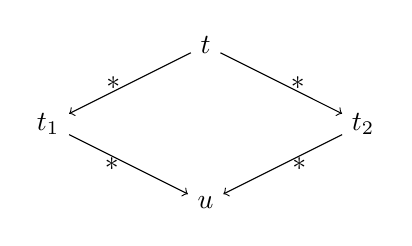
\begin{tikzpicture}	
  	\node(t) at (0,2) {$t$}; 
	\node(t1) at (-2,1) {$t_1$};
   	\node(t2) at (2,1) {$t_2$};
	\node (u) at (0,0) {$u$};
	\draw [->]  (t) --node[midway,left]{$*$} (t1) ;
	\draw [->]  (t) --node[midway,right]{$*$} (t2) ;
	\draw [->]  (t1) --node[midway,left]{$*$} (u) ;
	\draw [->]  (t2) --node[midway,right]{$*$} (u) ;
   \end{tikzpicture}
\end{figure} 
\end{block}
\end{frame}

\begin{frame}[fragile]{$\beta$-forma normal\u a}

Intuitiv, o form\u a normal\u a este  un termen care nu mai poate fi redus (sau punctul final al unui calcul). 

\begin{block}{Form\u a normal \u a}
\begin{itemize}
\item un $\lambda$-termen c\u aruia nu i se  mai poate aplica reducerea \^{\i}ntr-un pas $\ra_\beta$  se nume\sh te {\it $\beta$-form\u a normal\u a}
\item dac\u a $t\sra_\beta u_1$, $t\sra_\beta u_2$ \sh i $u_1$, $u_2$ sunt $\eta$-forme normale atunci, datorit\u a confluen\ts ei, $u_1=_\alpha u_2$
\item un $\lambda$-termen poate avea cel mult o $\beta$-form\u a normal\u a (modulo $\alpha$-echivalen\ts \u a)
\end{itemize}
\end{block}

\end{frame}

\begin{frame}[fragile]{$\beta$-forma normal\u a}

\begin{block}{Form\u a normal \u a}
\begin{itemize}
\item un $\lambda$-termen c\u aruia nu i se  mai poate aplica reducerea \^{\i}ntr-un pas $\ra_\beta$  se nume\sh te {\it $\beta$-form\u a normal\u a}
\item dac\u a $t\sra_\beta u_1$, $t\sra_\beta u_2$ \sh i $u_1$, $u_2$ sunt $\eta$-forme normale atunci, datorit\u a confluen\ts ei, $u_1=_\alpha u_2$
\item un $\lambda$-termen poate avea cel mult o $\beta$-form\u a normal\u a (modulo $\alpha$-echivalen\ts \u a)
\end{itemize}
\end{block}

Exemplu:
\begin{itemize}
\item $zv$ este $\beta$-form\u a normal\u a pentru  $(\lambda x.(\lambda y.yx)z)v$

$(\lambda x.(\lambda y.yx)z)v\ra_\beta (\lambda y.yv)z\ra_\beta zv$

\item exist\u a termeni care {\bf nu} pot fi redu\sh i la o $\beta$-form\u a normal\u a, de exemplu $(\lambda x. xx)(\lambda x. xx)$

\end{itemize}

\end{frame}


\begin{frame}[fragile]{$\beta$-conversia}

Intuitiv, $\beta$-conversia extinde $\beta$-reduc\ts ia \^{\i}n ambele direc\ts ii. 



\begin{itemize}
\item $(\lambda y. yv) z\ra_\beta zv \leftarrow_\beta (\lambda x.zx)v$\pause

\item $(\lambda y. yv) z\leftarrow_\beta (\lambda x.(\lambda y.yx)z)v \ra_\beta (\lambda x.zx)v$
\end{itemize}
\pause

\begin{block}{$\beta$-conversia  $=_\beta$}
\begin{itemize}
\item $=_\beta\subseteq \Lambda T\times \Lambda T$

$t_1=_\beta  t_2$ dac\u a  exist\u a $n\geq 0$ \sh i $u_0,\ldots, u_n$ astfel \^{\i}nc\^{a}t

$t_1=_\alpha u_0$, $u_n =_\alpha t_2$ \sh i, pentru orice $i$,
$u_i\ra_\beta u_{i+1}$ sau $u_{i+1}\ra_\beta u_{i}$

\end{itemize}
\end{block}

\pause

Exemplu: $(\lambda y. yv) z =_\beta (\lambda x.zx)v $
\end{frame}

\begin{frame}[fragile]{$\beta$-conversia}


\begin{block}{$\beta$-conversia  $=_\beta$}
\begin{itemize}
\item $=_\beta\subseteq \Lambda T\times \Lambda T$

$t_1=_\beta  t_2$ dac\u a  exist\u a $n\geq 0$ \sh i $u_0,\ldots, u_n$ astfel \^{\i}nc\^{a}t

$t_1=_\alpha u_0$, $u_n =_\alpha t_2$ \sh i, pentru orice $i$,
$u_i\ra_\beta u_{i+1}$ sau $u_{i+1}\ra_\beta u_{i}$

\end{itemize}
\end{block}\pause

\begin{block}{Observa\ts ii}
\begin{itemize}
\item $=_\beta$ este o rela\ts ie de echivalen\ts \u a\pause
\item pentru  $t_1$, $t_2$ $\lambda$-termeni \sh i $u_1$, $u_2$  $\beta$-forme normale 

dac\u a $t_1\sra_\beta u_1$, $t_2\sra_\beta u_2$ \sh i $u_1=_\alpha u_2$ atunci $t_1=_\beta t_2$
\end{itemize}
\end{block}

\end{frame}


\begin{frame}[fragile]{$\beta$-conversia}
\begin{block}{$\beta$-conversia  $=_\beta$}
\begin{itemize}
\item $=_\beta\subseteq \Lambda T\times \Lambda T$

$t_1=_\beta  t_2$ dac\u a  exist\u a $n\geq 0$ \sh i $u_0,\ldots, u_n$ astfel \^{\i}nc\^{a}t

$t_1=_\alpha u_0$, $u_n =_\alpha t_2$ \sh i, pentru orice $i$,
$u_i\ra_\beta u_{i+1}$ sau $u_{i+1}\ra_\beta u_{i}$

\item $=_\beta$ este o rela\ts ie de echivalen\ts \u a\pause
\item pentru  $t_1$, $t_2$ $\lambda$-termeni \sh i $u_1$, $u_2$  $\beta$-forme normale 

dac\u a $t_1\sra_\beta u_1$, $t_2\sra_\beta u_2$ \sh i $u_1=_\alpha u_2$ atunci $t_1=_\beta t_2$
\end{itemize}
\end{block}

\medskip

{\it $\beta$-conversia reprezint\u a "egalitatea prin calcul", iar $\beta$-reduc\ts ia (modulo $\alpha$-conversie) ofer\u a o procedur\u a de decizie pentru aceasta. }
\end{frame}

\begin{frame}{}
\vfill\begin{center}
\intens{Pe s\u apt\u am\^ana viitoare!}
\end{center}
\vfill
\end{frame}
\end{document}



